%This file contains all the Documentaion preamble settings and 
%font setting.


\documentclass[15pt]{article}

%-------------------------------------------
%use package
\usepackage[margin=1in]{geometry}
\usepackage{amsfonts, amsmath, amssymb}
\usepackage[none]{hyphenat}
\usepackage{graphicx}
\usepackage{float}
\usepackage{fancyhdr}
\usepackage{enumitem}
\usepackage[nottoc, notlot, notlof]{tocbibind}

%-------------------------------------------
%user define function
\def\blankpage{%
      \clearpage%
      \thispagestyle{empty}%
      \addtocounter{page}{-1}%
      \null%
      \clearpage}

%-------------------------------------------
%Define Page Style
\pagestyle{fancy}
\fancyhead{}
\fancyfoot{}
\fancyhead[L]{\uppercase{\textit{16x6 LED Matrix}}}
\fancyhead[R]{\textit{V1.0}}
\fancyfoot[C]{\thepage}

%-------------------------------------------
%Address for storing Images
\graphicspath{ {./images/} }

%-------------------------------------------
%user defined variables
\renewcommand{\footrulewidth}{2pt}
\parindent 0ex
%\setlength{\parindent}{4em}
%\setlength{\parskip}{1em}
\renewcommand{\baselinestretch}{1.5}
\newcounter{imageCounter}
\refstepcounter{imageCounter} %preamble of latex document
%List of Abbrevation 
\makenoidxglossaries


%Example - how to declare the acronym
%\newacronym{gcd}{GCD}{Greatest Common Divisor}
%\newacronym{lcm}{LCM}{Least Common Multiple}


%Example - How to use the acronym fucntions
%\acrlong{ } 
%Displays the phrase which the acronyms stands for. Put the label of the acronym inside the braces. In the example, \acrlong{gcd} prints Greatest Common Divisor.
%\acrshort{ } 
%Prints the acronym whose label is passed as parameter. For instance, \acrshort{gcd} renders as GCD.
%\acrfull{ } 
%Prints both, the acronym and its definition. In the example the output of \acrfull{lcm} is Least Common Multiple (LCM).


%MCU acronyms
\newacronym{mcu}{MCU}{Micro-controller Unit}
\newacronym{risc}{RISC}{Reduced Instruction Set Computer}
\newacronym{avr}{AVR}{Alf and Vegard's RISC}
\newacronym{io}{I/O}{Input and Output Line}
\newacronym{eeprom}{EEPROM}{Electrically Erasable Programmable Read-Only Memory}
\newacronym{sram}{SRAM}{Static Random Access Memory}
\newacronym{pwm}{PWM}{Pulse Width Modulation}
\newacronym{adc}{ADC}{Analog to Digital Converter}
\newacronym{usart}{USART}{ Universal Synchronous Asynchronous Receiver Transmitter}
\newacronym{spi}{SPI}{Serial Peripheral Interface}
\newacronym{i2c}{I2C}{Inter-Integrated Circuit}
\newacronym{gpio}{GPIO}{General Purpose Input and Output}
\newacronym{rx}{RX}{Receive Pin}
\newacronym{tx}{TX}{Transmit Pin}
%\newacronym{}{}{}

%Electronics hardware acronyms
\newacronym{led}{LED}{Light Emitting Diode}
\newacronyym{esd}{ESD}{Electro-Static Discharge}

%crystal acronyms
\newacronym{esr}{ESR}{Equivalent Series Resistance}
\newacronym{mhz}{MHz}{Mega Hertz}
\newacronym{khz}{KHz}{Kilo Hertz}
\newacronym{ppm}{ppm}{Parts Per Million}

%PCB acronyms 
\newacronym{pcb}{PCB}{Printed Circuit Board}
\newacronym{tht}{THT}{Through-Hole Technology}
\newacronym{smt}{SMT}{Surface Mount Technology}
\newacronym{smd}{SMD}{Surface Mount Devices}

%General acronyms
\newacronym{ble}{BLE}{Bluetooth Low Energy}
\newacronym{pc}{PC}{Personal Computer}
\newacronym{usb}{USB}{Universal Serial Bus}
\newacronym{ic}{IC}{Integrated Circuits}
\newacronym{kb}{KB}{Kilo Bytes}
\newacronym{lpf}{LPF}{Low Pass Filter}




 %acronym declaration file.

%-------------------------------------------
%Begin main document
\begin{document}
	
	
	\begin{titlepage}
		\begin{center}
			\vspace*{1cm}
			%\Large{\textbf{Transformer Power Supply}}
			\vfill
			\line(1,0){400}\\[1mm]
			\Huge{\textsc{Single Colour LED Matrix}}\\ [3mm]
			\huge{\textbf{-16x6 RED-}}\\ [1mm]
			\line(1,0){400}\\
			\vfill 
			\large{By : Ashwini Kumar Gupta\\
			B. Engg  Electronics \& Telecommunication\\}
			\today\\
			
		\end{center}
\end{titlepage}
	\blankpage
	
	%roman page numbering before Project Description	
	\pagenumbering{roman}
	
	\tableofcontents
	\thispagestyle{empty}
	\clearpage
	
	%\cleardoublepage
	%\addcontentsline{toc}{chapter}{\listfigurename}
	\listoffigures
	\clearpage
	
	\listoftables
	\clearpage
	
	%\chapter*{Declaration}
	%\addcontentsline{toc}{chapter}{Declaration}
	
	%\chapter*{Preface}
	%\addcontentsline{toc}{chapter}{Preface}
	
	\pagenumbering{arabic}
	\clearpage
	
	
	\vspace*{8.5cm}

\begin{minipage}{1.0\textwidth}

\begin{flushright}
	\section{\huge{\underline{Project Description}}}
\end{flushright}
\end{minipage}

%Multicols package is used to declate multiple %columns in the document class of latex
% \begin{multicols}{No. of COLUMNS} 
\begin{multicols}{2}

		\subsection{Introduction}
			Enter some text here.
			
		\subsection{Hardware}
			\subsubsection{MCU}
				The \textsc{led matrix} is built around a ATmega328P AVR microcontroller. This MCU is based on advanced RISC \cite{AtMega328P} architecture, 8 bit MCU and 23 programmable I/O lines. For controlling the \textsc{led matrix} shift registers are used, 2 for Column and 1 for row, due to shift registers few MCU I/O lines are used.
			\subsubsection{LED Matrix}
				 Single colour  RED 5mm LEDs used to build the matrix, total of 128 LEDs required for 16x8 matrix. An array of transistors configured as switch to provide required current for each row of LED matrix.  

			\subsubsection{Power supply}
				The project utilises a transformerless capacitive power supply design. Such a design is helpful in reducing the overall cost of project and also utilises fewer components thus saving space and cost.
				
				
			
			\subsubsection{Input}
				 The project is aimed to dynamically modify the display commands through an input source like PC or BLE. Such a feature helps in modifying the display at will rather than modifying the source code.

\end{multicols}

\begin{figure*}[h]		
	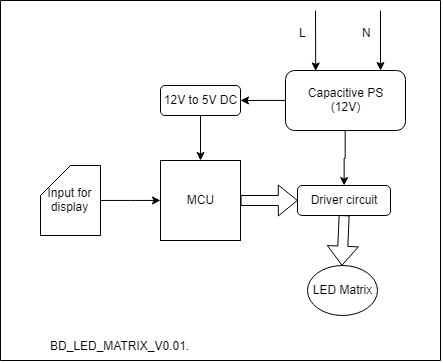
\includegraphics[scale = 0.3]{BD_LED_MATRIX_V1.png}
	\caption{Block Diagram V1.0}
	
\end{figure*}	
	
\begin{multicols}{2}

\end{multicols}	 
			
				  




	\blankpage
	
	
\vspace*{8.5cm}

\begin{flushright}
	\section{\huge{\underline{List Of Tools}}}
\end{flushright}

\subsection{Introduction}
	Enter some text here
	\blankpage
	
	\vspace*{8.5cm}

\begin{flushright}
	\section{Hardware}
\end{flushright}

\begin{multicols}{2}
	%start : PCBDesign/Introduction
%write between the comments
%%%%%%%%%%%%%%%%%%%%%%%%%%%%%%%%%%%%%%%%%%%%%%%%%%%%%%%%%%	
\subsection{Introduction}
	Enter some text here
	
%%%%%%%%%%%%%%%%%%%%%%%%%%%%%%%%%%%%%%%%%%%%%%%%%%%%%%%%%%	
%End : PCBDesign/Introduction
	
	\subsection{Control Unit}
	
	% Start - Hardware/Control Unit/MCU
%write Between the comments

\subsubsection{MCU}

	 \lettrine{T}{he} MCU is the central processing unit of the system. For this application/project the ATmega328P, by Atmel corporation, provides all the feature required. Following is the list of features \cite{AtMega328P}.
	 
	 \begin{itemize}
		\item Advanced RISC architecture
		\item 32K bytes of in-system self-programmable flash program memory.
		\item 1Kbytes EEPROM.
		\item 2Kbytes SRAM.
		\item Two 8-bit Timer/Counters
		\item One 16-bit Timer/Counter
		\item Six PWM channels
		\item 8-channel 10-bit ADC
		\item USART
		\item Master/slave SPI
		\item I2C
		\item watchdog timer
		\item On-chip analog comparator
		\item Six sleep modes 
		
		
	%	\begin{minipage}{0.3\textwidth}
	%		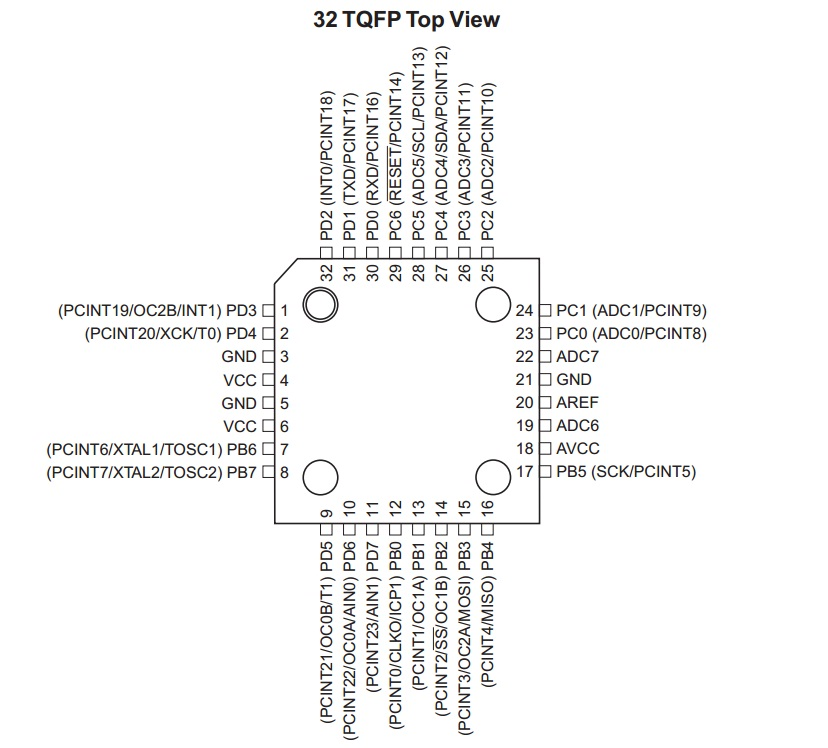
\includegraphics[width=\linewidth]{ATMega328p_TQFP_Pinout.jpg}
			%\caption{Block Diagram V0.21}
		%	\label{fig:image1}
			
		
		%\end{minipage}
		
	\end{itemize}	  
	 
	 

% End - Hardware/Control Unit/MCU

		
	% Start - Hardware/Control Unit/Oscillator Circuit
%write Between the comments


\subsubsection{Oscillator Circuit}
%first create all the reference in bibfile.

	\paragraph{The} oscillator circuit is required for generating clock for \gls{mcu}.Accuracy of timing application is dependent on the accuracy of the oscillator provided in the \gls{mcu}. The oscillators supported by ATmega328P are listed below \cite{AtMega328P}.
		\begin{itemize}
			\item Low power crystal oscillator
			\item \textbf{Full swing crystal oscillator}
			\item Low frequency crystal oscillator
			\item Internal 128 \gls{khz} RC oscillator
			\item Calibrated internal RC oscillator
			\item External clock
		\end{itemize}		
		
	\subparagraph{For }
	this application the \gls{mcu} will be in Full swing crystal oscillator mode.
	
	\subparagraph{\textbf{Advantages:}}
		
		\begin{itemize}
			\item 16 \gls{mhz}.
			\item rail to rail swing.
			\item Drive other clock sources
			\item Less effect of noisy environment 
		\end{itemize}		
	 
	 \subparagraph{Disadvantages:}
	 
	 	\begin{itemize}
	 		\item Higher current consumption than Low power crystal oscillator.(Power consumed by a crystal is not very significant, since using a 230 V AC source.)
	 		\item Operating Voltage of \gls{mcu} becomes 2.7 V to 5.00 V.(\gls{mcu} will be working on 5 V DC which is within the operating voltage defined.) 
		\end{itemize}	  	  
		
	\textbf{Selecting Crystal}
	
	\paragraph{Crystal Requirement}
	
		\begin{itemize}
			\item Frequency: 16 \gls{mhz}
			\item $C_{L}$: 6 - 11 pF \cite{AtMega328P}
			\item Mode of operation : Fundamental 
			\item Resonant: Parallel
			\item Tolerance: 0 - 50 \acrshort{ppm}
			\item Temperature Stability: 0 - 50 \acrshort{ppm}
			\item \gls{esr}: 60 to 100 $\Omega$
			\item Package type : \gls{smt} , since such crystals provide with less stray capacitance.
		\end{itemize}
	
	\paragraph{Selected Crystal} 
	is TSX-3225 16.0000MF09Z-AC0 a \gls{smt} 4 pin device package. Refer \ref{tab:selected_crystal} for details. 

	\subparagraph*{Oscillator Circuit Design}
	
		\begin{enumerate}
			\item \textbf{Load Cpacitors}:
			
				\begin{itemize}
					\item $C_{1}$ and $C_{2}$ together act as load capacitance.			
	
	\begin{figure}[H]
		\caption{Oscillator Circuit}
		\label{fig:crystal_circuit}
		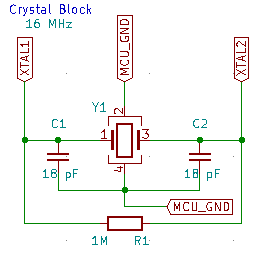
\includegraphics[scale=1]{crystal_ckt.png}
	\end{figure}

	\begin{table}[H]
		\caption{Crystal Properties(cite datasheet)}
		\label{tab:selected_crystal}
		\begin{tabular}{|r|c|}
				\hline
				\textbf{Device Manufacturer}                                                                            & \textbf{EPSON}                                                                            \\ \hline
				\textbf{Part No.}                                                                                       & \multicolumn{1}{l|}{\begin{tabular}[c]{@{}l@{}}TSX-3225 16.0000\\ MF09Z-AC0\end{tabular}} \\ \hline
				\textbf{Case (mm X mm)}                                                                                 & 3.2 x 2.5                                                                                 \\ \hline
				\textbf{\acrshort{tht} / \gls{smt}}                                        & SMD                                                                                       \\ \hline
				\textbf{\begin{tabular}[c]{@{}r@{}}Fundamental \\ Frequency ( \gls{mhz})\end{tabular}} & 16                                                                                        \\ \hline
				\textbf{\begin{tabular}[c]{@{}r@{}}Frequency \\ Stability (\acrshort{ppm})\end{tabular}}    & 9                                                                                         \\ \hline
				\textbf{\begin{tabular}[c]{@{}r@{}}Frequency \\ Tolerance(\acrshort{ppm})\end{tabular}}     & 10                                                                                        \\ \hline
				\textbf{$C_{L}$ pF}                                                                                     & 9                                                                                         \\ \hline
				\textbf{\begin{tabular}[c]{@{}r@{}}Operating\\ Temp max(\textdegree C )\end{tabular}}        & 75                                                                                        \\ \hline
				\textbf{\begin{tabular}[c]{@{}r@{}}Operating \\ Temp min(\textdegree C)\end{tabular}}        & -20                                                                                       \\ \hline
				\textbf{Aging (\acrshort{ppm})}                                                             & 1                                                                                         \\ \hline
				\textbf{ESR ($\Omega$)}                                                                                 & 60                                                                                        \\ \hline
		\end{tabular}
	\end{table}
	
	\item To have total 180\textdegree 	 shift due to active components (i.e capacitors), each capacitor provides with 90\textdegree  shift in phase. The value of the load capacitor is provided (cite datatsheet). 
	\item $C_{L}$ (Total Load capacitance) = 9 pF (cite DS)
	\item $C_{s}$ : Stray capacitance.
	\item $C_{1}$, $C_{2}$ are load capacitors
	\item Considering $C_{1} = C_{2}$. 
	\item value of $C_{1}$ and $C_{2}$ can be calculated using the following equation.
					\begin{align}				
						C_{L} &= {\frac{C_{1}C_{2} }{C_{1} + C_{2}}} + C_{s}\\
						C_{1} &= 2(C_{L} - C_{s})			
					\end{align}
	\item Considering $C_{s}$ = 0 pF.
					\begin{align}
						C_{1} &= 2(9 - 0)\\
						C_{1} &= 18 pF
					\end{align}
	\item Since crystal has drive level in range of 200 $\mu$ W, 0603 package ,i.e 0.1 W, is selected with value of 18 pF.
	\item The resistor $R_{1}$ is used to make the behaviour linear, this enhances the output of the crystal circuit. $R_{1}$ = 1 M $\Omega$, 0603.
				\end{itemize}
		
		\end{enumerate}		
	\paragraph{\gls{pcb} } design.
	

\cite{AVR042}

% End - Hardware/Control Unit/Oscillator Circuit 
	
	% Start - Hardware/Control Unit/Reset
%write Between the comments

\subsubsection{Reset}

	\paragraph{Reset}
	logic is used to set the \gls{mcu} in known state.The reset circuit for this \gls{mcu} is provided in figure \ref{fig:reset_circuit}.(cite avr042 here)
	
	\begin{figure}[H]
		\caption{Reset Circuit}
		\label{fig:reset_circuit}
		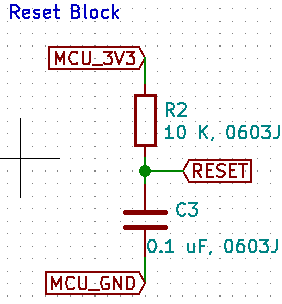
\includegraphics[scale=1]{reset_ckt.png}
	\end{figure}
	
	\textbf{Value Calculation}	
	\paragraph{R2}
	is acting as pull-up resistor here, which is used for high voltage programming (10V - 12V). Recommended value of pull-up resistor is 10 K$\Omega$.
	
	\paragraph{C3} 
	is used to filter high frequency noise, typical value is 100 nF (or 0.1 $\mu$F).
	
	\textbf{Power Calculation}
	
	Maximum allowable voltage for $V_{cc}$ is 5.5 V and $ V_{thresh}$ for reset pin detection is 1.1 V (cite datasheet here). 
	\begin{itemize}
		\item[R1:]
			\begin{align}
				n =m
			\end{align}
	\end{itemize}
	
%http://www.ti.com/interface/circuit-protection/esd-protection-and-tvs-surge-diodes/support-training.html
% End - Hardware/Control Unit/Reset
	
	%start : PCBDesign/programming
%write between the comments
%%%%%%%%%%%%%%%%%%%%%%%%%%%%%%%%%%%%%%%%%%%%%%%%%%%%%%%%%%	
\subsection{Programming}
	\subsubsection{USART}
		 Using male header 2x2 with (specify the dimension of male header) pin-out described in \ref{programming}.
		
	\subsubsection{\gls{icsp}}
		Using 2 x 3 male connector (specify the dimension of header) with pins as described in \ref{programming}
%%%%%%%%%%%%%%%%%%%%%%%%%%%%%%%%%%%%%%%%%%%%%%%%%%%%%%%%%%	
%End : PCBDesign/programming
	
	% Start - Hardware/Control Unit/Port Assignment
%write Between the comments

\subsubsection{Port Assignment}


% End - Hardware/Control Unit/Port Assignment
		
	% Start - Hardware/Control Unit/Voltage Level Indicator
%write Between the comments

\subsubsection{Voltage Level Indicator}


% End - Hardware/Control Unit/Voltage Level Indicator
	
	\subsubsection{Display Intensity controller}
	
	
		
	\subsection{Power Supply}
	
	\subsubsection{Power Switch}
	
	\subsubsection{Capacitive Power Supply}
	
	\subsubsection{Filter}
	
	\subsubsection{voltage Regulation}
	
	\subsubsection{Current Consumption}
	
	\subsection{LED Matrix}

	\subsubsection{LED}
	
	\subsubsection{Transistors}
	
	\subsubsection{Shift Registers}	
	
	\subsection{Input}	
\end{multicols}
	\blankpage
	
	
\vspace*{8.5cm}

\begin{flushright}
	\section{Software}
\end{flushright}

\subsection{Introduction}
	Enter some text here
	\blankpage
	
	\chapter{PCB Design}
	\blankpage
	
	
\vspace*{8.5cm}

\begin{flushright}
	\section{Mechanical CAD}
\end{flushright}

\subsection{Introduction}
	Enter some text here
	\blankpage
	
	%this document contains the appendix 
\appendix

\begin{multicols}{2}	
	%this section is only included inside the appendix and includes the crystal parameter definition in detail.
\section{Crystal}
		some text here
		
		\paragraph{Selecting} crystal requires following considerations.
		\begin{enumerate}
				\item \gls{tht} or \gls{smt}.
				\item Load capacitance.
				\item Frequency of operation
				\item Q - factor
				\item \gls{esr}
				\item Frequency Pulling
				\item Drive level
				\item Minimum negative Resistance
				\item Frequency stability
				\item Frequency Tolerance
		\end{enumerate}
		\blankpage
	
		
	\section{Title of app 22}
	some thext theri
	\blankpage
	
\end{multicols}
	
	\begin{multicols}{2}
		\printnoidxglossary[type=acronym]
    	\printacronyms
		\blankpage
		
		%Appendices
	
		
		%Refrences
		\bibliographystyle{ieee}
		\bibliography{bibfile}	
	
	\end{multicols}
	
\end{document}
%End main document